\documentclass[]{article}  

% Default font is the helvetica postscript font
\usepackage{helvet}
\usepackage{hyperref}
\usepackage{amsmath}
\usepackage{amsthm}
\usepackage{amssymb}
\usepackage[a4paper,margin=25mm]{geometry}
\usepackage{fancyhdr}
\usepackage{lipsum}
\usepackage[ruled,vlined]{algorithm2e}
\usepackage[utf8]{inputenc}
\usepackage[english]{babel}
\usepackage{graphicx}


\newtheorem{theorem}{Theorem}
\newtheorem{lemma}{Lemma}




%\renewcommand{\baselinestretch}{1.15}
\newcommand{\s}{\mathbf{s}}
\newcommand{\ba}{\mathbf{a}}
\newcommand{\bw}{\mathbf{w}}
\newcommand{\bx}{\mathbf{x}}
\newcommand{\bv}{\mathbf{v}}

\newcommand{\cA}{\mathcal{A}}
\newcommand{\cW}{\mathcal{W}}
\newcommand{\cH}{\mathcal{H}}

\newcommand{\R}{\mathbb{R}}
\newcommand{\E}{\mathbb{E}}
\newcommand{\h}{\mathbf{h}}
\newcommand{\KL}{\mathrm{D}_{KL}}
\newcommand{\thetab}{\mathbf{\theta}}


\title{PAC-Learnability of Half Lines: An Exact Proof}
\author{Behrad Moniri\\{\small Department of Electrical Engineering}\\{\small Sharif University of Technology}}
\date{}

\usepackage{sectsty} \sectionfont{\fontsize{15}{15}\selectfont}
\begin{document}

\maketitle
\begin{abstract}
	A careful proof of the PAC-Learnability of half lines is provided which unlike the standard textbook proofs, can handle distributions with atoms.
\end{abstract}
%\tableofcontents
%\section{* Exact Argument for PAC-Learnability of Half Lines}
\label{sec1}
In this note, we will prove the PAC learnability of the concept class $\mathcal{C} = \big\{[c, \infty): c\in\R\big\}$. In the proof mentioned in \cite{Schapire, mohri}, it is assumed that the probability measure has no atoms. Here we give a more general proof with no need to impose this assumption. Without loss of generality, assume that the true concept is $C = [0, \infty)$.


%In this proof, for every $I\subseteq \R$, we will denote $\mathbb{P}_{\bx\sim D}\big[||\bx|| \in I\big]$ as $\mathbb{P}[I]$ for simplicity.

%we need two conditions on $r_\epsilon$. First, the the probability $\mathbb{P}_{\bx\sim D}\Big[||\bx|| \in [r_\epsilon, r_c]\Big]$ should be small, to guarantee that that if our hypothesis meets the region, its error is small. Second, we need the probability $\mathbb{P}_{\bx\sim D}\Big[||\bx|| \in [r_\epsilon, r_c]\Big]$ to be large enough so that we will not miss it with high probability. It is readily evident that one should pay more attention to the constuction of $r_\epsilon$.

%\subsubsection{What is the problem?}

To state the proof, we first need to remind some basic properties of a probability measure.

\begin{lemma}
Any probability measure $\mathbb{P}$ satisfies the following properties:

\begin{itemize}
	\item \textbf{(Continuity from below)}: Let $E_1, E_2, E_3, \dots$ be measurable sets and $E_n \subseteq E_{n+1}$, for all $n$. The set $\bigcup_{i = 1}^{\infty} E_i$ is measureable and $\mathbb{P}\Big(\bigcup_{i = 1}^{\infty} E_i\Big) = \lim_{n\to \infty} \mathbb{P}[E_n]$.
	
	\item \textbf{(Continuity from above)}: Let $E_1, E_2, E_3, \dots$ be measurable sets and $E_{n+1} \subseteq E_{n}$, for all $n$. The set $\bigcap_{i = 1}^{\infty} E_i$ is measureable and $\mathbb{P}\Big(\bigcap_{i = 1}^{\infty} E_i\Big) = \lim_{n\to \infty} \mathbb{P}[E_n]$.
\end{itemize}

\begin{proof}
The proof can be found in every probability book such as \cite{grimmett}.
\end{proof}

\end{lemma}

Our proof is based on the following lemma.
\begin{lemma}
	\label{lem1}
	For fixed $\epsilon>0$ and probability measure $P$, set 
	$$h = \inf \Big\{h' : \mathbb{P}\big([0, h']\big)\geq\epsilon\Big\}.$$
	Let $R = [0, h]$ and $R' = [0, h)$. We have $\mathbb{P}[R'] \leq \epsilon$.
\end{lemma}

\begin{proof}
	Define $R_k = [0, k]$ and $R'_k = [0, k)$. The following statements trivially hold:
	\begin{itemize}
		\item $R_k' \subset R_k$.
		\item $a< b \implies R_a \subset R_b$.
		\item $k_n \uparrow h \implies \lim_{n\to \infty} R'_{k_n} = R'$.
	\end{itemize}
	By the definition of $h$, for any sequence $k_n \uparrow h$ we have
	$$\mathbb{P}[R'_{k_n}] \leq \mathbb{P}[R_{k_n}]<\epsilon.$$
	Thus, based on the continuity lemma, $\mathbb{P}[R'] = \lim_{n\to \infty}\mathbb{P}[R'_{k_n}] \leq \epsilon$.
\end{proof}

Now we are ready to prove our main result.

\begin{theorem} 
	The class $\mathcal{C} = \big\{[c, \infty): c\in\R\big\}$ is PAC-learnable.
\end{theorem}

\begin{proof}
Let $S$ be the set of samples and $C_S$ be the smallest half-line covering all positive samples. By construction, we have $C_S \subseteq C$. The means that we only have false negative errors and the region of error is exactly $\Delta = C - C_S$. If $\mathbb{P}[C] < \epsilon$, then $\mathbb{P}[C-C_S] < \epsilon$ and we are done. Hence, assume that $\mathbb{P}[C] \geq \epsilon$. Let $h = \inf \Big\{h' : \mathbb{P}\big([0, h']\big)\geq\epsilon\Big\}$, $R = [0, h]$, and $R' = [0, h)$. The following implication holds:
$$C_S\cap R \neq \emptyset \implies \Delta \subseteq R'.$$
Using Lemma \eqref{lem1}, we have $\mathbb{P}[R']\leq \epsilon$, hence
\begin{align}
\mathbb{P}[\mathrm{err}(C_S)>\epsilon]&\leq \mathbb{P}[C_S\cap R = \emptyset]\\
&=\mathbb{P}[S\cap R = \emptyset]\\
&= \big(1-\mathbb{P}(R)\big)^m.
\end{align}
Note that, $\mathbb{P}(R)\geq \epsilon$, so $1 - \mathbb{P}(R) < 1- \epsilon$. The reason for this is the countinuity lemma and converging to $R$ using an increasing sequence from inside. Thus we can write
\begin{align}
\mathbb{P}[\mathrm{err}(C_S)>\epsilon]&\leq \big(1-\mathbb{P}(R)\big)^m\\
&\leq (1-\epsilon)^m \leq e^{-m\epsilon}.
\end{align}
Setting $\delta$ to be greater or equal to the right hand side, yields $m \geq \frac{1}{\epsilon}\log\Big(\frac{1}{\delta}\Big)$.
\end{proof}

\bibliography{bib}
\bibliographystyle{ieeetr}

\end{document}

Note that from now, we will assume the probability measure has no atoms. The proofs can all be modified by a similar argument as the one give above for the more general case.



\section{Learning Circles}

This problem is very similar to the question discussed in class. Let $S$ be our sample set of size $m$ and $A$ be the our learning algorithm. Given a sample set $S$, the output of $A$ is the smallest circle containing all samples with positive label. The radius of $A(S)$ is denoted by $r_S$. Also let $c$ be the concept, which is a circle with radius $r_c$, $\epsilon>0$ be an arbitrary positive real number, and $D$ be a distribution on $\mathbb{R}^2$. Construct the ring region $[r_\epsilon, r_c]$ such that $\mathbb{P}\Big[||\bx|| \in [r_\epsilon, r_c]\Big] = \epsilon$. These regions can be constructed by starting with the empty ring along a the of $c$ and increasing its size until its distribution mass is at least $\epsilon$. For a more rigorous treatment, please see section \eqref{sec1}. The circle $c_\epsilon$ with radius $r_\epsilon$ is a slightly smaller circle compared to $c$.  Error occurs if a point is in the region between $A(S)$ and $c$. 
\begin{figure}[h!]
	\centering
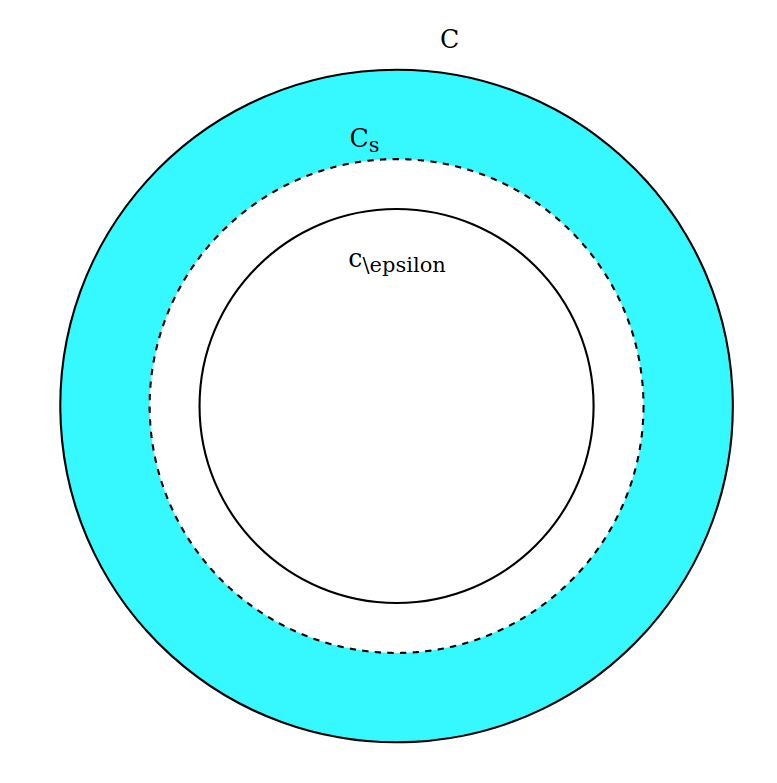
\includegraphics[scale=0.25]{./fig/circle.png}
\caption{The circles $C$, $C_S$ and $C_\epsilon$ are plotted in this figure. The error region is marked with blue.}
\end{figure}

The generalization error of $A(S)$ is

$$L_D(c_S) = \mathbb{P}_{\bx\sim D}\Big[||\bx|| \in [r_S, r_c]\Big]. $$

\noindent
From the definition of $r_\epsilon$, we know that 
$$r_S \in [r_\epsilon, r_c] \implies L_D(c_S)\leq \epsilon,$$
Thus we can write
\begin{align*}
\mathbb{P}[L_D(c_S)> \epsilon] &\leq \mathbb{P}\Big[r_S \notin [r_\epsilon, r_c]\Big]\\
&\leq \mathbb{P}\Big[\text{no points in } [r_\epsilon, r_c]\Big]\\
&\leq \prod_{i = 1}^{m} \mathbb{P}\Big[\text{sample } i \text{ not in } [r_\epsilon, r_c]\Big]\\
&\leq (1-\epsilon)^m \leq e^{-m\epsilon}.
\end{align*}
Setting $\delta$ to be greater or equal to the right hand side, yields $m \geq \frac{1}{\epsilon}\log\Big(\frac{1}{\delta}\Big)$.


\section{Learning Rectangles and Cubes}

\subsection{Rectangles}

Let $R$ be the concept, $S$ be the sample set, and $R' = A(S)$ be the smallest axis-aligned rectangle containing all samples with positive label and $\epsilon$ be an arbitrary positive real number.


Define four rectangle regions along the sides of $R$, each with probability at least $\frac{\epsilon}{4}$. These regions can be constructed by starting with the empty rectangle along a side and increasing its size until its distribution mass is at least $\frac{\epsilon}{4}$. 


\begin{figure}[h!]
	\centering
	\begin{minipage}{.5\textwidth}
		\centering
		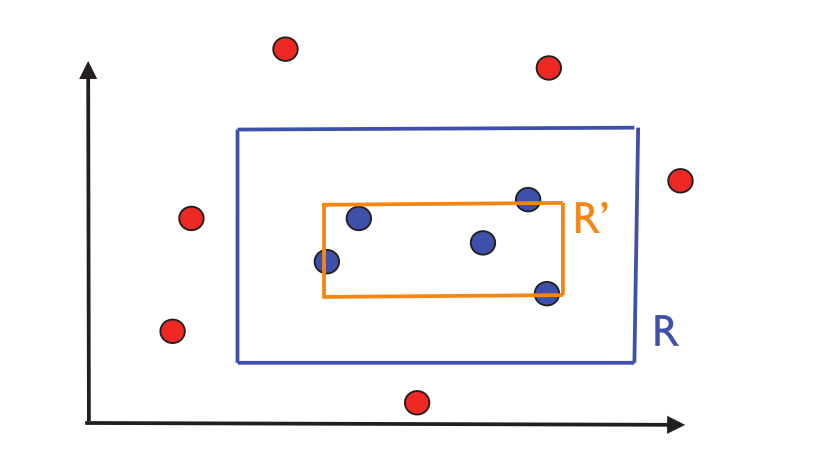
\includegraphics[scale=0.24]{./fig/RectPAC.png}
	\end{minipage}%
	\begin{minipage}{.5\textwidth}
				\centering
		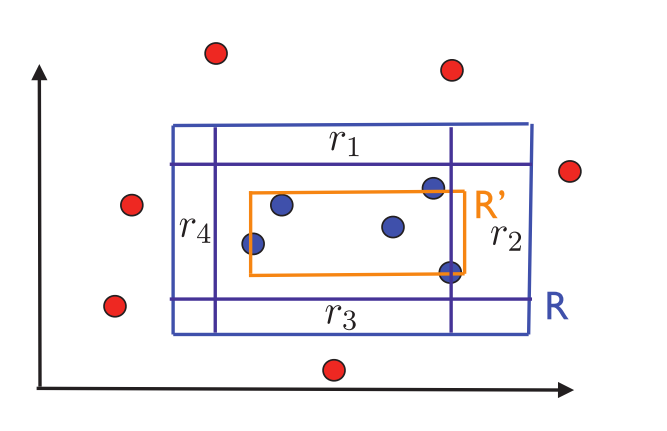
\includegraphics[scale=0.27]{./fig/RectPAC2.png}
	\end{minipage}
\caption{The true rectangle $R$, hypothesis $R_S = R'$, and small rectangles $r_i$.}
\end{figure}


\noindent
The following geometric implication holds:
$$\text{There is a sample in each of the four small rectangles } \implies L_D(R')\leq \epsilon.$$
Hence, 
\begin{align*}
	\mathbb{P}\Big[L_D(R') > \epsilon\Big] &\leq \mathbb{P}\Big[\text{There exists a small rectangle with no samples in it}\Big]\\
	&= \mathbb{P} \Big[ \bigcup_{i = 1}^{4} \{\text{no sample in rectangle } r_i\}\Big]\\
	&\leq \sum_{i = 1}^{4} \mathbb{P}\Big[\{\text{no sample in rectangle } r_i\}\Big]\\
	&\leq 4\big(1-\frac{\epsilon}{4}\big)^m\leq 4e^{-m\frac{\epsilon}{4}}.
\end{align*}
Setting $\delta$ to be greater or equal to the right hand side, yields $m \geq \frac{4}{\epsilon}\log\Big(\frac{4}{\delta}\Big)$.


\subsection{Hypercube}
Hypercubes are very similar to rectangles! Consider $2d$ small hypercubes, each with probability at least $\frac{\epsilon}{2d}$.  These regions can be constructed by starting with the empty hypercube along a side and increasing its size until its probability measure is at least $\frac{\epsilon}{2d}$. Following the exact same steps as above, we arrive at $m \geq \frac{2d}{\epsilon}\log\Big(\frac{2d}{\delta}\Big)$. The sample complexity, increase with rate $d\log(d)$ as the dimension increases.

\subsection{Noisy Rectangle}

Please note that this problem does not fit completely within the PAC framework. Consider the rectangle problem again. We will mimic the arguments here. We can still write the following implication:
$$\text R'\text{ misses non of the regions } r_i \implies L_D(R')\leq \epsilon.$$
Hence, we can still upper bound the probability of having large error as follows:
\begin{align*}
\mathbb{P}\Big[L_D(R') > \epsilon\Big] &\leq \mathbb{P}\Big[R' \text{ misses at least one of the regions } r_i \Big]\\
&\leq \sum_{i = 1}^{4} \mathbb{P}\Big[\{R' \text{ misses region } r_i\}\Big]
\end{align*}
\noindent
Each term can be bounded as follows:

\begin{align*}
\mathbb{P}\Big[\{R' \text{ misses region } r_i\}\Big] &= \prod_{i = 1}^{m}\mathbb{P}\Big[x_i \text{ not in } r_i \text{ or it is in } r_i \text{ but label is flipped.}\Big]\\
&\leq  \prod_{i = 1}^{m}\Big(\mathbb{P}\Big[x_i \text{ not in } r_i\Big] + \mathbb{P} \Big[x_i \text{ is  in } r_i \text{ but label is flipped.}\Big]\Big)\\
&\leq \Big(1-\frac{\epsilon}{4} + \frac{\eta\,\epsilon}{4}\Big)^m \\
&\leq \Big(1-\frac{\epsilon}{4} + \frac{\eta'\,\epsilon}{4}\Big)^m \\
&= \Big(1-\frac{\epsilon}{4} (1-\eta')\Big)^m \leq \exp\Big(-\frac{m\epsilon}{4}(1-\eta')\Big) 
\end{align*}
Thus, 
\begin{align*}
\mathbb{P}\Big[L_D(R') > \epsilon\Big] &\leq 4\exp\Big(-\frac{m\epsilon}{4}(1-\eta')\Big).
\end{align*}
Setting $\delta$ to be greater or equal to the right hand side, yields $m \geq \frac{4}{(1-\eta')\epsilon}\log\Big(\frac{4}{\delta}\Big)$.


\section{Learning Intervals}
This is a special case of a hypercube with $d=1$.

\section{Learning Union of Intervals}

First, consider $p=2$ for simplicity. Consider the following algorithm.

\begin{algorithm}[H]
	\SetAlgoLined
	\KwIn{Sample set $S = \{(x_1, y_1), \dots, (x_m, y_m)\}$.}
	

	Sort samples based on their $x$ value.
	
	Mark the interval of consecutive positive labeled samples.
	
	\KwOut{Union of intervals matching the start and end samples in each interval found above.}

	\caption{Learning Union of Intervals}
\end{algorithm}

\vspace{0.5cm}
\noindent
Let our concept be $I = [a, b] \cup [c, d]$ in which $a<b<c<d$. The are two events of error:
\begin{itemize}
	\item False positive in $(b, c)$.
	\item False negative in $[a, b]$ or $[c, d]$. 
\end{itemize}
We have seen the false negative error in previous examples. The false positivity happens if we have no sample in $(b, c)$. We can now formally quantify these quantities. Let $h_s$ be the output of our algorithm, given sample set $S$. Formally, 
\begin{align*}
	L_D(h_S) &= \mathbb{P}[x \in h_S, x \notin I] + \mathbb{P}[x \notin h_S, x \in I]\\
	&= \underbrace{\mathbb{P}[x \in h_S, x \notin I]}_{L_{FP}} + \underbrace{\mathbb{P}\big[x \notin h_S, x \in [a,b]\big]}_{L_l} +  \underbrace{\mathbb{P}\big[x \notin h_S, x \in [c,d]\big]}_{L_r}.
\end{align*}
We know how to control $L_r$ and $L_l$, hence we reduce our problem to a problem involving bounding these quantities:
\begin{align*}
\mathbb{P}[L_D(h_S) > \epsilon] \leq \mathbb{P}\Big[L_{FP} > \frac{\epsilon}{3}\Big] + \mathbb{P}\Big[L_l > \frac{\epsilon}{3}\Big]+ \mathbb{P}\Big[L_r > \frac{\epsilon}{3}\Big].
\end{align*}
Now lets focus on false positivity. As mentioned earlier, this error happen if there is no sample in $(b, c)$. Note that  $L_{FP} > \frac{\epsilon}{3} \implies \mathbb{P}\Big[(b, c)>\frac{\epsilon}{3}\Big]$. Hence, 

$$L_{FP} = \mathbb{P}\Big[L_{FP} > \frac{\epsilon}{3}\Big] \leq \big(1-\frac{\epsilon}{3}\big)^m \leq \exp\Big({-\frac{m\,\epsilon}{3}}\Big).$$
We now turn our attention to $L_r$ and $L_l$. These two can be bounded using the same method as previous question
\begin{align*}
 \mathbb{P}\Big[L_{l} > \frac{\epsilon}{3}\Big] \leq 2 \exp\Big(\frac{-m\,\epsilon}{6}\Big),
\hspace{1cm} 
 \mathbb{P}\Big[L_{r} > \frac{\epsilon}{3}\Big] \leq 2 \exp\Big(\frac{-m\,\epsilon}{6}\Big).
\end{align*}
Summing up, we have 
$$\mathbb{P}\Big[L_D(h_S)>\epsilon\Big] \leq  4 \exp\Big(\frac{-m\,\epsilon}{6}\Big) +\exp\Big({\frac{-m\,\epsilon}{3}}\Big) \leq 5\exp\Big({\frac{-m\,\epsilon}{6}}\Big). $$
Setting $\delta$ to be greater or equal to the right hand side, yields $m \geq \frac{6}{\epsilon}\log\Big(\frac{5}{\delta}\Big)$.

This result can be easily generalized to an arbitrary $p$ as the regions are treated independently in the proof. In this case, there are $p$ false positive and $2p$ false negative regions. Thus, 
$$\mathbb{P}\Big[L_D(h_S)>\epsilon\Big] \leq  2p \exp\Big(\frac{-m\,\epsilon}{2(2p-1)}\Big) + (p-1)\exp\Big({\frac{-m\,\epsilon}{2p-1}}\Big) \leq (3p-1)\exp\Big({\frac{-m\,\epsilon}{2(2p-1)}}\Big). $$
Setting $\delta$ to be greater or equal to the right hand side, yields $m \geq \frac{2(2p-1)}{\epsilon}\log\Big(\frac{3p-1}{\delta}\Big)$. 


Note that the sample complexity increases with rate $p \log (p) $ as $p$ grows. The time complexity of the algorithm is $O(m\log(m))$, because of the sorting subroutine.
\end{document}